\documentclass[smallextended,natbib]{svjour3}       % onecolumn (second format)
\usepackage{graphicx}
\usepackage{todonotes}
\usepackage{url}
\usepackage{lineno}
\linenumbers

\begin{document}
	
%opening
\title{Pikunda-Munda and Batalimo-Maluba}
\subtitle{Archaeological Investigations of the Iron Age Settlement History of the western and northern Congo Basin}
%\titlerunning{Short form of title}        % if too long for running head

\author{}
%\author{Dirk Seidensticker}

%\institute{Dirk Seidensticker \at
%	Ghent University \\
%	Department of Archaeology \\
%	UFO, Sint-Pietersnieuwstraat 35 \\
%	B-9000 Ghent \\
%	\email{dirk.seidensticker@ugent.be}
%}

\date{Received: date / Accepted: date}
% The correct dates will be entered by the editor

\maketitle

\begin{abstract}
The spread of pottery-producing communities into the Central African rainforest is commonly linked to the so-called ‘Bantu Expansion’. It is considered the primary linguistic, cultural, and demographic process in Holocene sub-Saharan Africa. To describe the expansion of putative Bantu-speech communities through the rainforest into southern Africa, substantial migrations through the so-called ‘Sangha River Interval’, which mostly coincides with the Sangha River valley, are proposed. This paper presents a coherent picture of the archaeological settlement history in the western and northern Congo Basin, uncovered by fieldwork of the late 1980s along the rivers Ngoko, Sangha, Likwala-aux-Herbes, Ubangi, and Lua. Archaeological research of the \textit{River Reconnaissance Project}, directed by Manfred K. H. Eggert from 1977 to 1987, produced a pottery sequence for the Congo Basin. Archaeological features and findings uncovered during the project’s field campaigns in the northern and western Congo Basin have only recently been studied in detail. Due to a total lack of subsequent archaeological fieldwork in this region, this analysis provides the only reliable source for a reconstruction of the cultural dynamics within the region. Archaeological data and the sequence of pottery styles within the western Congo Basin, along the Sangha River, cannot support the claim that this region, due to a climate-induced extension of savannas, played a unique role as a ‘corridor’ within the expansion of putatively ‘Bantu’ speaking groups during the latter half of the 1st millennium BCE.

\noindent\textbf{Résumé} La propagation des communautés productrices de poteries dans la forêt tropicale d'Afrique centrale est généralement liée à ce que l'on appelle "l'expansion bantoue". Elle est considérée comme le principal processus linguistique, culturel et démographique de l'Afrique subsaharienne holocène. Pour décrire l'expansion des communautés de langue bantoue présumées à travers la forêt tropicale jusqu'en Afrique australe, on propose des migrations importantes à travers ce que l'on appelle " l'intervalle de la rivière Sangha ", qui coïncide principalement avec la vallée de la rivière Sangha. Cet article présente une image cohérente de l'histoire du peuplement archéologique dans l'ouest et le nord du Bassin du Congo, mise au jour par les travaux de terrain de la fin des années 1980 le long des rivières Ngoko, Sangha, Likwala-aux-Herbes, Ubangi et Lua. Les recherches archéologiques du \textit{River Reconnaissance Project}, dirigé par Manfred K. H. Eggert de 1977 à 1987, ont produit une séquence de poterie pour le Bassin du Congo. Ce n'est que récemment que les caractéristiques et les découvertes archéologiques mises au jour lors des campagnes de terrain du projet dans le nord et l'ouest du Bassin du Congo ont été étudiées en détail. En raison de l'absence totale de travaux archéologiques ultérieurs dans cette région, cette analyse constitue la seule source fiable pour une reconstruction de la dynamique culturelle de la région. Les données archéologiques et la séquence des styles de poterie dans l'ouest du Bassin du Congo, le long de la rivière Sangha, ne peuvent pas soutenir l'affirmation selon laquelle cette région, en raison d'une extension des savanes induite par le climat, a joué un rôle unique en tant que " corridor " dans l'expansion des groupes parlant prétendument " bantou " au cours de la dernière moitié du 1er millénaire avant notre ère.

\keywords{Congo Basin \and Pottery \and Iron Age \and Settlement History}
\end{abstract}

\section*{Introduction}\label{intro}

The archaeological sequence in the Inner Congo Basin or Cuvette central has been studied in detail \citep{Wotzka.1995}, while finds from the adjacent western and northern fringes of the Central African rainforest were only recently analyzed \citep{Seidensticker.2021e}. The region is critical because prevailing models of the spread of a sedentary lifestyle, regularly derived from linguistic reconstructions of modern languages, propose them as routes of substantial migrations at the onset of the so-called ‘Bantu-Expansion’ \citep{Bostoen.2018,Bostoen.2020}. Historical linguists offered two main models to describe the variability of modern languages that are part of the Bantu language family: an 'early split' of languages with predicted migrations on the northern fringes of the rainforest and a ‘late split’ model with migrations through the rainforest and subsequent diversification. Evolutionary genetic research on modern communities points towards demic diffusion as the driving force behind the expansion of Bantu languages in favor of the distribution of languages and technologies \citep{Bostoen.2022,Pakendorf.2011}. Relying on phylogenetic modeling and coupling their results with evolutionary genetic research, historical linguists favor rapid expansion into and through the equatorial forests \citep{Currie.2013,Bostoen.2015,Grollemund.2015,Koile.2022,Grollemund.2023}. Regularly these findings are coupled with the intensification of archaeological remains yielding ceramics and dating into the 1st millennium BCE \citep{deSaulieu.2021a,Seidensticker.2021}. Subsequently, such approaches induce ‘procedural puzzles’ and fail at linking linguistics with “the authentic material evidence of archaeology” \cite[88]{Eggert.2016a}. However, only archaeological research can provide discrete historical data on the cultural processes within Central Africa before the second half of the 15th century CE.

\subsection*{History of Research}

Between 1977 and 1987, extensive boat surveys along the tributaries of the Congo River were performed in the context of the River Reconnaissance Project, directed by Manfred K. H. \cite{Eggert.1983,Eggert.1984,Eggert.1993,Eggert.1996}. A summary of this project’s discoveries in the Inner Congo Basin, south of the Congo river, has been published by Hans-Peter \cite{Wotzka.1993}. Wotzka’s reconstruction of the settlement history of the Cuvette central relies on a sequence of 35 pottery-style groups that span the last two-and-a-half millennia and comprises six stylistic traditions. The initial phase dates from 400 to 200 BCE and is represented by the pottery of the Imbonga style \citep[59--68]{Wotzka.1995}. The expansion continued into the 16th century CE, and the first settlers did not penetrate the entire region at once. Instead, the Inner Congo Basin settling followed multiple successive waves of upriver expansions \citep[226-–241]{Wotzka.1995}. \cite[290]{Wotzka.1995} concludes that “the explored parts of the Inner Congo Basin constitute a remarkably self-containing ceramic sphere in the course of the last 2 400 years” and that “all [encountered] pottery styles could be traced back to the Imbonga group”. Aiming at uncovering the northern extent of the Imbonga style, fieldwork of the River Reconnaissance Project in 1985 was extended along the Ubangi river and its tributary, the Lua river \citep{Eggert.1987c}. The survey covered the tropical rainforest up to the tropical savanna (Fig.~\ref{fig:map}). The roughly 850~km long exploration of the Ubangi yielded 44 sites, of which only the site of Motenge-Boma has been known previously \citep[75]{vanNoten.1978,vanNoten.1982a}. Four additional sites were discovered along an approximately 100~km long stretch of the lower Lua River, most notably Maluba, where multiple pit features were excavated. Along the Lobaye River, a tributary of the Ubangi, the renowned site of Batalimo remains the only other site in the region that produced a distinct record like that of Maluba dating back to the earliest settlement of the region. The site was first discovered in 1966 during construction works, and a 2x3 m big trench was excavated in 1968 \citep{deBayledesHermens.1975}. The site was revisited in 1981 by Pierre Vidal and most notably by Lassina Koté between 1987 and 1990 \citep{Kote.1992}. More recent excavations directed by Alfred Jean-Paul Ndanga focused on examining the cultural layer discovered by \cite{deBayledesHermens.1975}, which contains partially polished lithic artifacts and ceramics. \cite[137]{Eggert.1987c} questions the inventory's coherence based on this research at Maluba.

After the surveys along the Ubangi and Lua, which did not yield pottery associated with the earliest styles from the Inner Congo Basin, the campaign of 1987 focused on the western parts of the Congo Basin \citep{Eggert.1992}. More precisely, the northern part of the Republic of Congo. The nearly 600~km long survey of the Sangha River, from its mouth at Mossaka – around 220~km south of Mbandaka – up to Bomasa at the border triangle of the Republic of the Congo, Cameroon, and the Central African Republic, yielded 38 new sites (Fig.~\ref{fig:map}). A survey along a roughly 80~km long stretch of the Ngoko River, which joins the Sangha north of Ouesso, added another eight sites. The last survey, the River Reconnaissance Project conducted in 1987, covered the Likwala-aux-Herbes river, which runs in-between the Ubangi and Sangha and is characterised by a very distinct ecology \citep{Philippon.2019}. The Likwala-aux-Herbes, not to be confused with the Likwala-Mossaka running further west, is characterised by a swampy bush- and grassland. Higher vegetation only appears multiple kilometres away from the river. Thus, a vast floodplain can be found at each river bank, unlike along the Sangha River, where the rainforest vegetation reaches directly to the river bank. The 530 km long survey yielded another 23 sites. The entire region surveyed in 1987 was archaeological \textit{terra incognita} before. The project’s discoveries, including preliminary results from the western and northern Congo Basin, were outlined in a well-known paper concerning the archaeology of the equatorial rainforest \citep{Eggert.1993}. The survey and excavation finds were partially summarized \citep{Seidensticker.2016b} until the detailed analysis was published recently \citep{Seidensticker.2021e}. 

Fieldwork in the region re-commenced during the past decade. Contrasting earlier endeavours is the prevalent integration of paleo-ecological research. Focal points of research have been the Ngoto forest reserve in the south-eastern parts of the Central Africa Republic \citep{Kiahtipes.2011,Lupo.2015,Kiahtipes.2016,Lupo.2021}, the northern parts of the Republic of the Congo \citep{Gillet.2013,MorinRivat.2014,Morin-Rivat.2017a}, the north-eastern parts of the Congo Basin \citep{Cornelissen.2013,LivingstoneSmith.2011,LivingstoneSmith.2017}, as well as the Inner Congo Basin \citep{Neumann.2022}.

\begin{figure*}[!tb]
	\includegraphics[width=\textwidth]{fig/fig_map.pdf}
	\caption{Map of the Congo Basin. White dots are known sites with pottery finds (dark dots representing sites mentioned in the text). Green shading shows the modern extent of the equatorial rainforest \citep{White.1983}. Dark green shading represents the putative extent (refugia) of the rainforest during the 1st millennium BCE rainforest crisis \citep{Bremond.2017,Maley.2017}. The purple dotted line shows the extent of the Congo Basin \citep[11]{Runge.2001}. Grey shading show topography above 500 m ASL.}
	\label{fig:map}
\end{figure*}

\begin{table*}[!tb]
	\includegraphics[width=\textwidth]{tbl/Tab_New14C.pdf}
	\caption{Calibrated ages of newly obtained AMS dates obtained from the inside of pottery sherds and stable isotope values. All previously published radiocarbon dates can be found in the online aDRAC repository \cite{Seidensticker.2021f}.}
	\label{tab:14C}	
\end{table*}

\subsection*{Study Area: Landscape and Geography}

The paper’s study area is a north-south transect through the rainforest, as most surveyed rivers run north to south. It covers the tropical savanna climate (‘Aw’-climate according to the Köppen-Geiger systematic) in the north, followed by the tropical monsoon climate (‘Am’), while the bulk of sites is located in tropical rainforest climate (‘Af’) \citep{Peel.2007}. At the heart of the study area lies the Congo Basin, which is dominated by the Congo River and its many tributaries. The catchment area of the Congo river covers the entire area of the Democratic Republic of the Congo (DRC) as well as large parts of the Republic of the Congo, south-eastern Cameroon, southern Central African Republic and adjacent areas further east, south-east and south of the DRC \citep[60 Fig. 1]{Eggert.2017}. The Congo Basin is generally limited to a topography below 450 m ASL \citep[11]{Runge.2001} with quaternary geological deposits \citep{Persits.1997}.
 
For this review of the settlement processes, the study area is represented best when subdivided into the “western Congo Basin” (rivers Ngoko, Sangha and Likwala-aux-Herbes) and the “northern Congo Basin” (region of the Ubangi and Lua River) (Fig.~\ref{fig:map}).

\section*{Materials and Methods}\label{materials}

The research is based on inventories of 122 sites along the rivers Ubangi, Lua, Sangha, Ngoko, and Likwala-aux-Herbes (Fig.~\ref{fig:map}). The study area covers an area of about 500\,$\times$\,700 km. In total, the studied collection is comprised of around 10.500 individual objects, including roughly 4.200 vessel units and a similar amount of highly fragmented ceramic sherds \citep[23--43]{Seidensticker.2021e}. At five sites, 14 features were excavated. Most of the excavated features were pits. Additional pit features were sampled at four sites. Only about a third of the studied ceramics was discovered during excavations of deliberate sampling of clearly identifiable features.

Morphologically and ornamentally similar vessel units are summarised as pottery styles, following the established conceptualizations of \cite[52--57]{Wotzka.1995}. The styles describe a specific and recognizable way ceramics are produced and decorated. Additionally, early investigations into clay sourcing, conceptualized as macroscopic pottery fabrics \citep[60--69]{Seidensticker.2021e}, were included in the morphological description of ceramic sherds and vessels.

The study’s main objective was to develop a spatiotemporal reference framework for the area based on pottery groups derived from the ceramics' technological, morphological, and ornamental characteristics. Twenty-four new ceramic style groups were described for the northern and western Congo basin combined. Furthermore, five styles found mainly within the Inner Congo basin and described by \cite{Wotzka.1995} could be identified.

Established concepts were adopted (\citeauthor{Eggert.1983} \citeyear{Eggert.1983}, 295; \citeyear{Eggert.1984}, 250, 257; \citeyear{Eggert.1988}, 28--31; \citeauthor{Wotzka.1995} \citeyear{Wotzka.1995}, 217--225) to describe the change and development of pottery with the study area. A sequence of subsequent pottery styles that share clear indications that one was derived of the other are regarded as ‘pottery traditions’ or ‘style tradition’ \citep{Rouse.1957,Willey.1945}, while contemporaneous sets of closely related pottery styles are summarized as ‘style horizon’ \citep[108--111]{Kroeber.1944}.

All data and computer code produced are available here: \url{https://github.com/dirkseidensticker/PikundaMunda_BatalimoMaluba_AAR}

\subsection*{Radiocarbon Dating}

In total, 21 conventional radiocarbon samples were dated in the 1980s. All those dates were conducted conventionally and on charcoals found within the features. Two additional samples from bone material were AMS dated in 2014 \citep[355--356 Appendix 2]{Seidensticker.2021e}. All dates are available via the aDRAC online repository \citep[\url{https://github.com/dirkseidensticker/aDRAC};][]{Seidensticker.2021f} and thus not listed individually here. Four samples obtained off food crusts from the interior of ceramics were AMS dated, providing for the first time direct and precise dates associated with the usage of the pottery (Tab.~\ref{tab:14C}). Stable carbon and nitrogen isotopes were also measured to compensate for fresh-water reservoir effects.

\begin{figure*}[!tbp]
	\centering
	\includegraphics[width=\textwidth]{fig/fig_bayesphases.pdf}
	\caption{Alpha distributions of Bayesian phase models for the duration of pottery styles \citep{Crema.2020a,Crema.2021a} that are dated via at least two reliable radiocarbon dates.}
	\label{fig:bayes}
\end{figure*}

\begin{table*}[!tbp]
	\centering
	\includegraphics[width=.75\textwidth]{tbl/tbl_bayesphases_comparison.pdf}
	\caption{Comparison between conventional start and end dates for radiocarbon dated pottery groups in the Congo Basin \citep[Data S2]{Seidensticker.2021} and median start and end calendar years derived from Bayesian phase determination (Fig.~\ref{fig:bayes}).}
	\label{tab:bayes}
\end{table*}

\subsection*{Bayesian Phase Modeling}

The previously determined chronological ranges of the pottery groups \citep{Seidensticker.2021e, Seidensticker.2021} were further examined using Bayesian phase modeling. While \cite{Crema.2020a} relied on the OxCal software to run their model, an implementation that is available via the nimbleCarbon R-package was used \cite{Crema.2021a,Crema.2021b}. The code used to define the model was derived of the vignette provided with the nimbleCarbon software. A simple Bayesian chronological model was fitted to those radiocarbon dates that showed sufficient archaeological contextualization and have not been discarded as potential lab errors in prior studies \cite[9]{Seidensticker.2021} for each pottery style to recover posterior probabilities for its onset and end (Fig.~\ref{fig:bayes}). To compare these with the conventional estimations provided in earlier studies \cite[\url{https://github.com/dirkseidensticker/aSCAC};][Data S2]{Seidensticker.2021}, the median age value of the posterior distribution was extracted (Tab.~\ref{tab:bayes}).

\section*{Results}

\subsection*{Early Iron Age (200 BCE – 500 CE) in the Western Congo Basin}

\subsubsection*{Imbonga style}

Remnants of the oldest ceramics in the western Congo Basin are found at two sites along the lower Sangha River, at Mitula and Mobaka \citep[Fig.~\ref{fig:map};][169--172, 306--307]{Seidensticker.2021e}. At both villages, fragments of diagnostic vessels were found partially embedded in the soil, indicating eroded remains of pit features. During the pottery's extraction, charcoal was found and subsequently radiocarbon dated. Charcoal from inside the vessel at Mobaka dates to the 8th to 1st centuries BCE (KI-2894), while the sample from underneath the vessel at Mitula dates to the 6th to 1st centuries BCE (KI-2895; Fig.~\ref{fig:chrono}). Both conventional radiocarbon dates show substantial standard errors and thus cover long timespans after calibration. These dates correspond to the age of the Imbonga style, dated to the 4th to 1st centuries BCE and constituting the initial phase of settlement history in the Congo Basin \citep[Fig.~\ref{fig:bayes}; \ref{fig:chrono}; Tab.~\ref{tab:bayes};][59--68]{Wotzka.1995}. The Imbonga style is characterized by vessels with flat bases that either show round bellies, pronounced shoulders, and profiled rims or are wide-mouthed bowls. Its decoration patterns comprise of rocker-stamping on the lower half, often combined with horizontal grooves and incised or plastic ornamentation on the vessels' shoulder regions. The two mentioned vessels found on the lower Sangha river do not represent classic Imbonga characteristics but show striking similarities to vessels associated with the Imbonga style: the vessel found at Mitula resembles another from Iyonda \citep[441 Pl.~7.7]{Wotzka.1995} while the vessel from Mobaka matches one found at Bokele \citep[453 Pl.~19.10]{Wotzka.1995}. These relatively isolated finds indicate an area of influence the Imbonga group had west of its previously known boundary.

\begin{figure*}[!tb]
	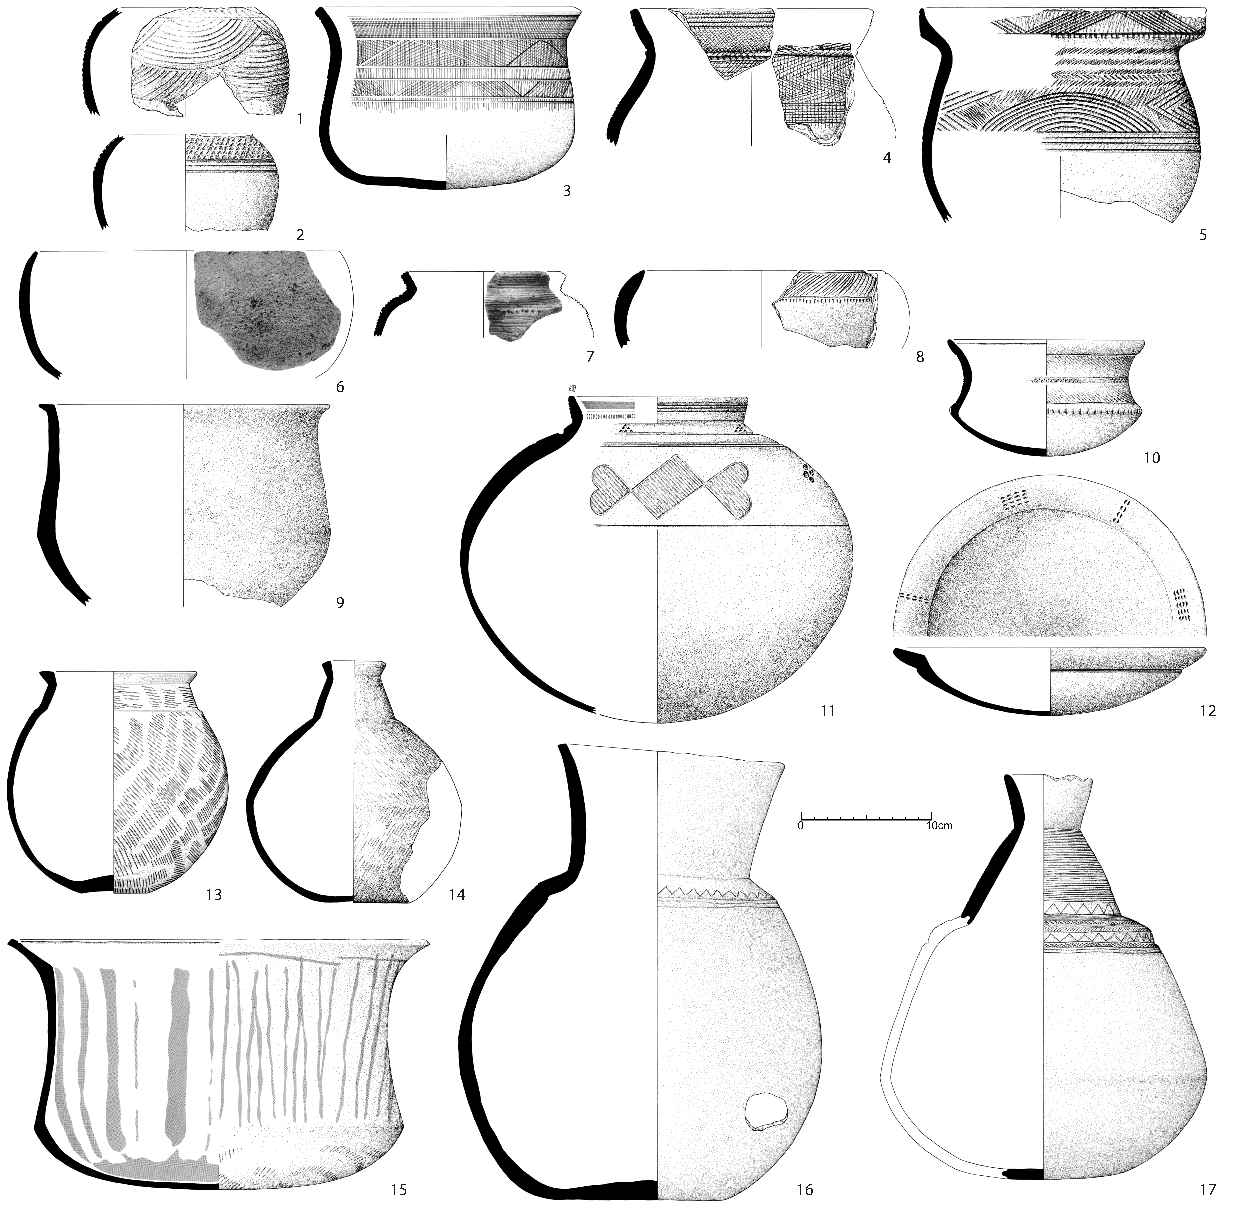
\includegraphics[width=\textwidth]{fig/Sangha_Typen.pdf}
	\caption{Ceramic vessels from the western Congo Basin -- along the rivers Ngoko, Sangha and Likwala-aux-Herbes -- that are representative for the following pottery styles: 1--3) Pikunda-Munda; 4) Bokonongo; 5--7) Bobusa; 8 \& 10--11) Ngombe; 9) Matoto; 12--13) Ebambe; 14) Mobaka; 15-16) Epena \citep[114--144, 162--168]{Seidensticker.2021e}.}
	\label{fig:sangha}
\end{figure*}

\subsubsection*{Pikunda-Munda style}

The Pikunda-Munda group represents the earliest pottery style in the western parts of the Congo Basin \citep[114-120]{Seidensticker.2021e}. It shows substantial similarities to the contemporaneous groups in the Inner Congo Basin regarding pottery technology and decorations. However, concerning vessel shapes, there are considerable differences \citep[107 Ftn.~4]{Wotzka.1995}. The Pikunda-Munda style is represented best through the inventories of pit features excavated in 1987 at the two eponymous sites: Pikunda on the middle Sangha River and Munda on the upper Likwala-aux-Herbes River (Fig.~\ref{fig:map}). The excavation at Pikunda detected two features: one about 3.4~m deep pit dating from the 4th century BCE to the 3rd century CE (KI-2877; RICH-30864; Tab.~\ref{tab:14C}) that's been intersected by a considerably younger pit \citep[288--300]{Seidensticker.2021e}. The older pit contained two nearly complete vessels and around 160 sherds that can be attributed to the Pikunda-Munda style, as well as one rim sherd of the Lusako style known from the Inner Congo Basin (\citeauthor{Eggert.1992} \citeyear{Eggert.1992}, 18 Fig.~4.1; \citeauthor{Wotzka.1995} \citeyear{Wotzka.1995}, 104–-107). Four sherds show a considerably different fabric, shape and decoration similar to that of the Ngbanja style known from the middle Ubangi river \citep[296 Tab.~34]{Seidensticker.2021e}. At Munda, two pits and a metallurgy-related feature yielded inventories of the Pikunda-Munda style \citep[321--339]{Seidensticker.2021e}. All features dated between the 1st century BCE and 4th century CE (Fig.~\ref{fig:bayes}; \ref{fig:chrono}, Tab.~\ref{tab:bayes}). The inventories from these pits are quite different compared to the one excavated at Pikunda, whose pottery is heavily fragmented. The pits at Munda contained complete vessels intentionally deposited either upside-down or lying on their side; a practice reminiscent of the depositions in pits in the Inner Congo Basin \citep{Wotzka.1993}. Overall nearly 550 vessel units are attributed to the Pikunda-Munda group, with two-thirds of the assemblage originating from the excavations mentioned above at the two eponymous sites.

Pikunda-Munda pottery was found along the Sangha River from its mouth into the Congo River in the south up to the village of Ikelemba, around 65~km southeast of Ouesso, and along the entire stretch of the Likwala-aux-Herbes River \citep[Fig.~\ref{fig:timeslices};][119 Fig.~49]{Seidensticker.2021e}. A vessel from Ingonda Bosopela along the lower Lulonga river \citep[119 Ftn. 4, 531 Pl. 97.5]{Wotzka.1995} and a few isolated sherds found southeast and northeast of Ouesso \citep[114 Fig.~42]{Gillet.2013} can be attributed to the Pikunda-Munda style as well.

The main characteristic of the Pikunda-Munda pottery are wide, open-mouthed bowls with approximately cylindrical walls, flared rims and rounded bases \citep[Fig.~\ref{fig:sangha}:1--3;][311--314]{Eggert.1993}. Ornamental motives are based on linear elements produced through incisions or grooves, as well as occasional rocker-stamp decoration \citep[362 Appendix 4.12]{Seidensticker.2021e}. Utilizing of these decoration techniques and motives corresponds to contemporaneous practices in the Inner Congo Basin. Especially concerning their decoration, there are considerable similarities between the Pikunda-Munda style and the styles Lokondola, Lusako, Lingonda, and Bokuma \citep[107]{Wotzka.1995}. The main difference to the contemporaneous ceramics of the Inner Congo Basin is that among Pikunda-Munda pottery, only round bases are observed, while the ceramics further east unanimously show flat bases.

Irrespective of these morphological differences, pottery technology of the Pikunda-Munda ceramics and pottery from the Inner Congo Basin are practically indistinguishable. Their fabrics indicate that they are made from fine river clays with no temper added \citep[66--67 Fig.~21]{Seidensticker.2021e}. The used clays proved to be rich in sponge spicules \citep{Seidensticker.2020}. A small-scale pilot study on their shaping techniques showed that Pikunda-Munda vessels are roughed out by a version of drawing of a ring technique, and thus in a very similar fashion as pottery production observed in the late 1970s and early 1980s at Ikenge in the Inner Congo Basin \citep{Eggert.1980c}.

The oldest feature in the Congo Basin associated with iron metallurgy thus far pertains to the Pikunda-Munda group: the upper part of a pit at Munda on the upper Likwala-aux-Herbes River contained 7.5 kg of iron slag partially embedded in a hard-fired clay lining \citep[321--330]{Seidensticker.2021e}. The features also contained five nearly complete Pikunda-Munda bowls deposited laying on their sides \citep[323 Fig.~157.A--E; Pl.~91.1--5]{Seidensticker.2021e}. Two radiocarbon dates from that part of the feature date into the 1st to 4th centuries CE (KI-2885, KI-2887).

Neither the precursor nor a potential successor of the Pikunda-Munda pottery is known. The precise association between the Pikunda-Munda style and contemporaneous styles of the Equator-Co style tradition remains a subject for subsequent research. The present state of knowledge points to the Pikunda-Munda group being a sub-stream of the \textit{Equator-Co} style tradition and no independent entity.

\subsubsection*{Other Finds}

Several vessels from a partially eroded pit on the banks of the Likwala-aux-Herbes (Kilometer 186) have no comparison in the region in terms of vessel shapes and decorations \citep[165--168, 339--340]{Seidensticker.2021e}. Time constraints during fieldwork only allowed a quick sampling of the pit, obtaining a nearly complete vessel, four larger fragments and 13 smaller sherds (\citeauthor{Eggert.1993} \citeyear{Eggert.1993}, 320 Fig.~16.15; \citeauthor{Seidensticker.2021e} \citeyear{Seidensticker.2021e}, Pl. 76.1--11). A charcoal sample dates this features between the 2nd century BCE to the 3rd century CE (KI-2893). The vessel has a flat base, convex belly, and a slightly elaborated shoulder leading to a concave neck and a flared rim. Its decoration consists of crudely made crossing grooves made with a comb on the shoulder and impressions beneath the rim. Further fragments show similar decorations. Overall, the vessel's shape is substantially different from those of the contemporaneous Pikunda-Munda style. Some aspects of the ceramics resemble a vessel found at Gbadolite on the upper Ubangi river \citep[277-278 Fig. 7]{Eggert.1984}. Nevertheless, the only accurate comparison for its shape, decoration technique and motives can be found among pottery of the Ngovo group in the lower Congo region \citep{deMaret.1986}.

The Bokonogo style is an interim term for an inventory of 19 vessel units from seven sites, including Pikunda on the middle Sangha River, that show very distinct characteristics: all vessels are either rather tall with convex bellies and concave necks ending in cylindrical rims or bowls with inverted rims \citep[Fig.~\ref{fig:sangha}.4;][120--123]{Seidensticker.2021e}. Decorations consist of grooves beneath the rim and on the neck and shoulders, mainly forming horizontal, chevron or crossing motives. About half of the inventory showed a fabric similar to that of the Pikunda-Munda group, while a quarter showed grog tempering. At the same time, the remainder contained a heterogenous mix of quartz and grog. All finds are surface finds and not associated with any indications of their dating. The only accurate comparison in terms of morphological characteristics and decorations can be found among the Oveng pottery found in north-western Gabon \citep[615--618]{Clist.20042005} and on the island of Corisco (Equatorial Guinea) (\citeauthor{GonzalezRuibal.2011} \citeyear{GonzalezRuibal.2011}; \citeyear{GonzalesRuibal.2012}; \citeauthor{SanchezElipe.2015} \citeyear{SanchezElipe.2015}, 217--221; \citeauthor{SanchezElipe.2016} \citeyear{SanchezElipe.2016}, 351--355). Oveng ceramics date from the 2nd century BCE to the 5th century CE \citep[555 Fig. 7–14]{Clist.20042005}. The resemblance provides a provisional chronological estimate for the Bokonongo pottery to date around the first half of the 1st millennium CE (Fig.~\ref{fig:chrono}).

Close to the mouth of the Sangha river, in the very south of the study area, a unique kind of pottery was found that is characterized by predominant grog tempering and small globular pots with short everted rims or convex bowls with slightly inverted rims \citep[Fig.~\ref{fig:sangha}.5--7;][162--165]{Seidensticker.2021e}. This group is named after the site of Bobusa, located near the mouth of the Sangha river. While there are no radiocarbon dates available for this pottery group, some of its characteristics show similarities to pottery found on the Île des Mimosas in Kinshasa that is dated into the 2nd to 4th centuries CE \citep[279--280]{Eggert.1984}. This timespan is provisionally also proposed as the age of the Bobusa pottery (Fig.~\ref{fig:chrono}).

\subsection*{Early Iron Age (200 BCE – 500 CE) in the Northern Congo Basin}

The 1985 survey along the Ubangi River from its mouth into the Congo River south of Mbandaka up to Kouango and along the Lua river (Fig.~\ref{fig:map}) yielded a first glimpse into the variability of ceramics in the northern parts of the Congo Basin. The distribution of pottery groups in the northern Congo Basin is separated into three distinct regional lines of development \citep[183--185]{Seidensticker.2021e}: on the lower part of the river, up to 180 to 240~km upstream, all observed ceramics are part of the Equator-Co tradition of the Inner Congo Basin. Inventories from sites in that region are dominated by the newly described Bokwango style and the already established styles Bondongo, Mbandaka, and Botendo \citep[96--98, 172--181]{Seidensticker.2021e}. All these groups are dated into the late Iron Age. The area further upstream, up to Bangui, showed a complex set of pottery styles described below. Upstream of Bangui, only pottery associated with the Late Iron Age has been identified as of yet.

\begin{figure*}[!tb]
	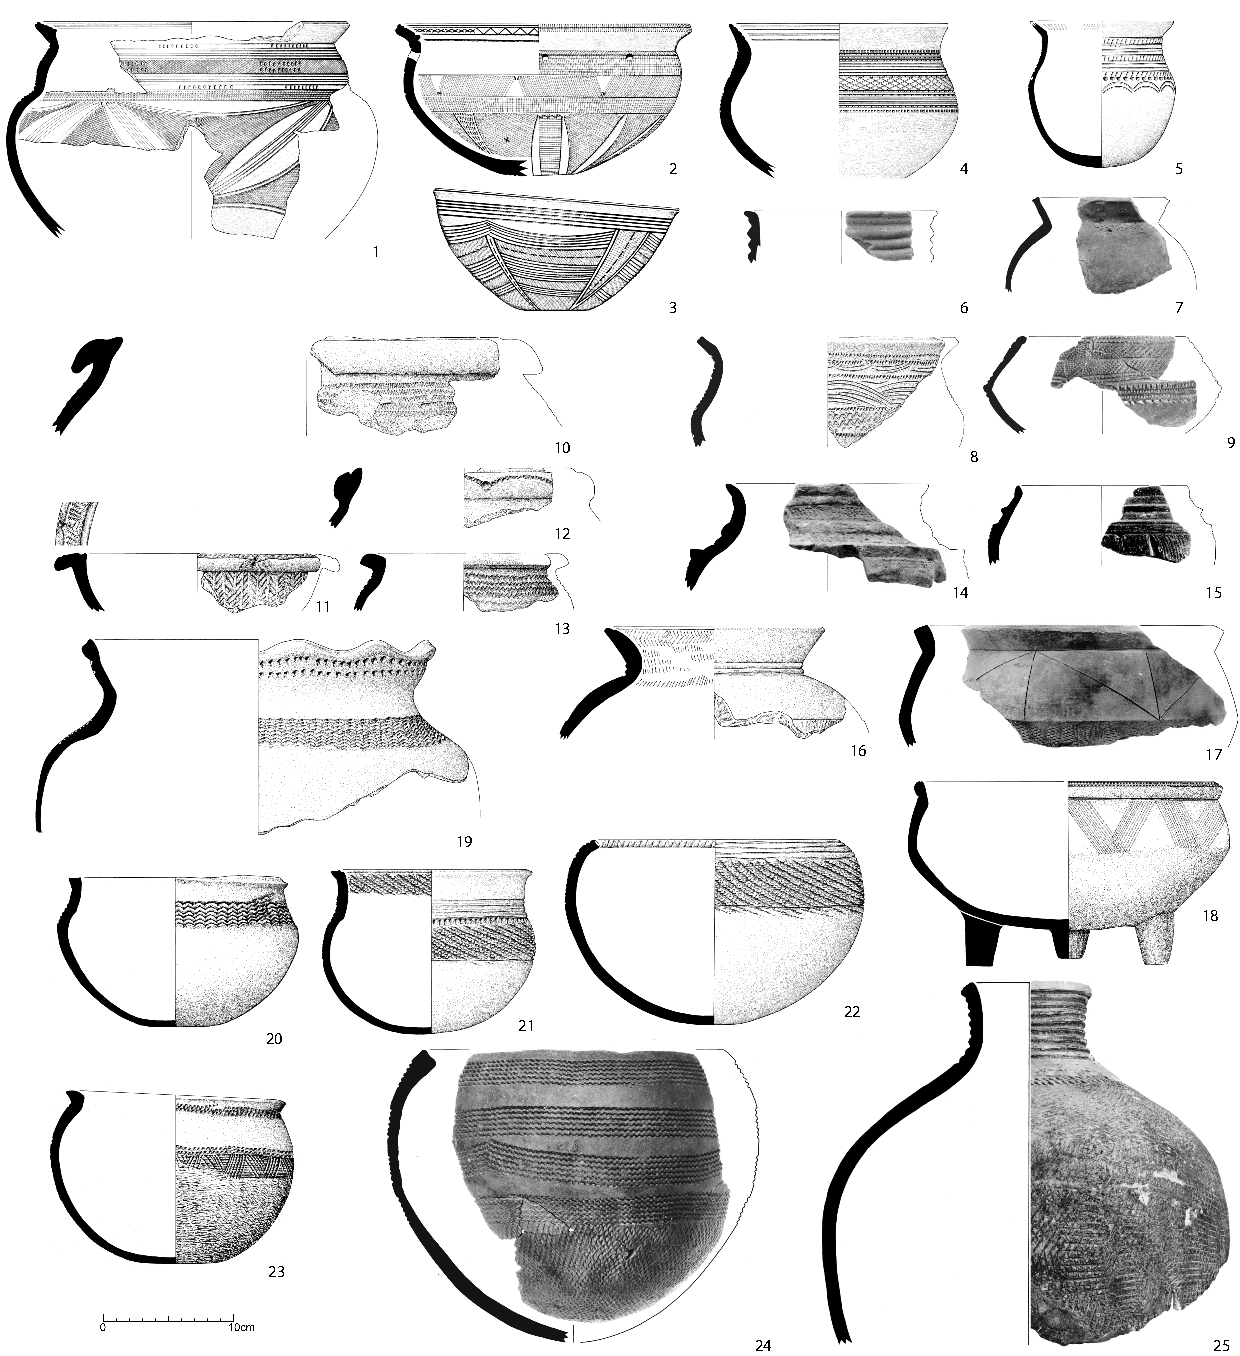
\includegraphics[width=\textwidth]{fig/Ubangi_Typen.pdf}
	\caption{Ceramic vessels from the northern Congo Basin -- along the rivers Ubangi and Lua -- that are representative for the following pottery styles: 1--3) Batalimo-Maluba; 4--5) Ngbanja; 6--7) Bobulu; 8--9) Mokeke; 10--11) Bokwango; 12--15) Motenge-Boma; 16--17) Mbati-Ngombe; 18--19) Dama; 20) Bangui; 21) Kpetene \citep[75--114]{Seidensticker.2021e}.}
	\label{fig:ubangi}
\end{figure*}

\subsubsection*{Batalimo-Maluba style}

In the region between Impfondo and Bangui, henceforth referred to as the middle Ubangi river, the ceramic sequence starts with the Batalimo-Maluba style \citep[75--82]{Seidensticker.2021e}, named after the eponymous sites Batalimo on the lower Lobaye river and Maluba on the lower Lua river (Fig.~\ref{fig:map}). Excavations at Batalimo were conducted by \cite{deBayledesHermens.1975}, Vidal, \cite{Kote.1992} and \cite{Ndanga.2010}. The initial excavation indicated a coexistent of partially polished lithic artifacts and ceramics \citep{Aumassip.1975}. This was not supported by later excavations at the site \citep{Ndanga.2010}, nor excavations at the other eponymous site Maluba \citep{Eggert.1987c}. The pottery of the Batalimo-Maluba style was found at 18 sites, with a core distribution area between Dongo near the mouth of the Lua River and Mokelo, about 30~km downstream of Bangui. The most southern find was uncovered at Ngbanja near Impfondo \citep[Fig.~\ref{fig:timeslices};][81 Fig.~25]{Seidensticker.2021e}. Only in Batalimo and Maluba excavations yielded pottery of this style. The other sites associated with this group originate from surface finds. Available radiocarbon dates and one thermoluminescence date (OxTL-154a-4), indicate that the Batalimo-Maluba pottery dates between the 2nd century BCE and 6th century CE \citep[Fig.~\ref{fig:bayes}; \ref{fig:chrono}; Tab.~\ref{tab:bayes};][80 Fig.~28]{Seidensticker.2021e}. 

Batalimo-Maluba pottery is characterized by well-structured, flat-based globular pots and wide-mouthed bowls that are elaborately decorated using cross-hatching, impression motifs and incised or grooved lines organized in alternating horizontal and vertical zones (Fig.~\ref{fig:ubangi}.1--3; \citeauthor{Eggert.1993} \citeyear{Eggert.1993}, 306--308; \citeauthor{Seidensticker.2016b} \citeyear{Seidensticker.2016b}, 118; \citeyear{Seidensticker.2021e}, 75--82).

\subsubsection*{Nbganja style}

Closely related to the Batalimo-Maluba style is the Ngbanja style, which shares similar general characteristics \citep[82--86]{Seidensticker.2021e}. The primary vessel types are globular or slightly ovaloid pots or beakers with everted rims (Fig.~\ref{fig:ubangi}.4--5). Decorations are based on grooves and impressions, and while they show similar motives as the Batalimo-Maluba style, they are restricted to the neck or inside of the rim.

Ngbanja pottery is strongly related to the Batalimo-Maluba style, and Eggert (\citeyear{Eggert.1987c}, 141) suggested it as a predecessor of the Batalimo-Maluba group. Besides the stylistic connections, the only chronological fixpoint for the Ngbanja style is a sherd of this style found in the deep pit at Pikunda (Sangha river). Two radiocarbon dates (KI-2877, RICH-30864; Tab.~\ref{tab:14C}) date the feature to the second half of the 1st century BCE to the late 3rd century CE. The sherd exhibits a coarse fabric instead of the delicate fabric common to the Pikunda-Munda style, and its decor consists of a ledge with comb impressions on it. A nearly matching sherd was found during surveys at Ngbanja on the middle Ubangi river \citep[83 Fig.~26.7--8]{Seidensticker.2021e}. At Pikunda, this sherd must be considered a foreign but contemporaneous type within the closed Pikunda-Munda inventory. Three other sherds with coarse fabric and a decoration different from the Pikunda-Munda style were also found. These associations allow for the possibility that Ngbanja pottery is contemporaneous not only to Batalimo-Maluba pottery but also to the Pikunda-Munda style and dates between the 2nd/1st century BCE and the 5th/6th century CE (Fig.~\ref{fig:chrono}; \ref{fig:timeslices}).

\subsection*{Middle Iron Age (500--1000 CE) in the Congo Basin}

In both regions, inventories dating between the end of the 6th century to the early 10th century CE are currently unknown, leaving a gap within the regional sequences of at least 300 years (Fig.~\ref{fig:bayes}; \ref{fig:chrono}; \ref{fig:timeslices}). A detailed review of chronological indicators for the 32 pottery styles described by Wotzka (\citeyear{Wotzka.1995}, 59--212) revealed that no pottery could be dated between the end of the Bokuma and Lingonda styles, which end towards the end of the 7th centuries CE, and the onset of the widespread Bondongo style at the beginning of 12th century CE (Fig.~\ref{fig:bayes}; Tab.~\ref{tab:bayes}).

In the north-eastern Congo Basin, around Kisangani (Fig.~\ref{fig:map}), a similar interruption between ceramics designated to the Early and Middle Pottery Phase and styles pertaining to the Late Iron Age has been observed \citep[Fig.~\ref{fig:bayes}; \ref{fig:chrono};]{LivingstoneSmith.2017}. Technological analyses of the shaping techniques revealed a distinction as well: the pottery of the Early and Middle phases is exclusively shaped via a drawing of a ring technique, while all Late Iron Age pottery is shaped by pounding in a concave mold. Only certain stages of the \textit{chaînes opératoires} of the Late Iron Age ceramics still adhere to principles followed during earlier times, indicating a certain continuity (pers. comm Livingstone-Smith 2021).

Two recent papers firmly established a supra-regional pattern of putative demographic changes in Central Africa during the past three millennia \citep{deSaulieu.2021a,Seidensticker.2021}.

\subsection*{Late Iron Age (1000--1850 CE) in the Western Congo Basin}

After the interruption of pottery sequences during the Middle Iron Age, ceramics re-appear within the archaeological inventories of the region in the 11th century CE (Fig.~\ref{fig:bayes}; \ref{fig:chrono}; \ref{fig:timeslices}). During the late Iron Age in the western Congo Basin, a clear distinction appears between pottery styles associated with the adjacent Inner Congo Basin and an independent stream summarized as Ngoko style tradition.

\subsubsection*{Ngombe style}

The re-emergence of ceramics in the western Congo Basin at the onset of the Late Iron Age is marked by the Ngombe style \citep[125--128]{Seidensticker.2021e}, which is rooted in the Equator-Co tradition of the Inner Congo basin \citep[222 Fig. 4]{Wotzka.1995}. The ceramics of this type are found mainly on the lower Sangha river, with the eponymous site of Ngombe constituting the northernmost extension of its distribution area \citep[127 Fig. 54]{Seidensticker.2021e}. In total, 56 vessel units from 15 sites are associated with the Ngombe style. They are similar to the Longa and Mbandaka styles \citep[121--128, 139--143]{Wotzka.1995} of the Inner Congo Basin but show equally independent characteristics. The defining inventory of the Ngombe style was discovered in a partially eroded pit feature at the eponymous site on the middle Sangha river \citep[305-–306, Pl.~42.15--44.2]{Seidensticker.2021e}. It yielded an inventory of two plates, a big bowl, and a carinated bowl, all surrounded by fragments of a large vessel with a convex belly, a tapered shoulder and a short, flared rim \citep[Fig.~\ref{fig:sangha}.8,10--11;][Pl. 42.15--44.2]{Seidensticker.2021e}. The Ngombe style shows only rounded bases. Decorations consist of grooves and impressions on the upper parts of the vessels. A new radiocarbon date obtained off a food crust from the bottom of the main vessel found at Ngombe dates into the late 12th to mid-13th century CE (RICH-30867; Tab.~\ref{tab:14C}). This corroborates the previously proposed age of this pottery in relation to the Mbandaka and Longa styles of the Inner Congo Basin \citep[Fig.~\ref{fig:bayes}, \ref{fig:chrono}, \ref{fig:timeslices}; Tab.~\ref{tab:bayes};][126--128]{Seidensticker.2021e}. 

\subsubsection*{Ebambe and Epena styles}

Modern pottery production in the western Congo Basin shows two styles being present along the Likwala-aux-Herbes river: upstream dominates the Epena style, while downstream, the Ebambe style is more present, but with vessels of both styles being found along the entire length of the river \citep[131--141]{Seidensticker.2021e}. Only the Ebambe style has been found along the lower Sangha River. A potter in Boleko, on the lower Likwala-aux-Herbes river, was still producing pottery of the Ebambe style in 1987 using a drawing of a lump technique combined with additional coiling for the neck \citep{Eggert.inVorb.}. Defining vessel shapes are tall vessels with tapered necks, bottles with think necks and bowls with parallel rims \citep[Fig.~\ref{fig:sangha}.12--13;][132 Fig.~57]{Seidensticker.2021e}. All vessels of the Ebambe style show flat bases. A diagnostic feature of the Ebambe style is the consistent use of \textit{bnfwa-nfwa} decor on nearly all parts of the vessel, including occasionally the inside of the rims. A rich inventory of Ebambe-style vessels was excavated in Munda on the upper Likwala-aux-Herbes river \citep[311--321]{Seidensticker.2021e}. New radiocarbon dates on food crusts from two vessels found within the pit (RICH-30865, RICH-30866; Tab.~\ref{tab:14C}) corroborate the existing convention date (KI-2884). All three dates cover the 16th century CE onwards.

The pottery produced at Epena on the upper Likwala-aux-Herbes river shares similar morphological features with the Ebambe style, especially their flat bases and tall vessels with tapered necks \citep[Fig.~\ref{fig:sangha}.15--16;][137--141]{Seidensticker.2021e}. Production was documented in 1995 by Léopold Mpika Ngoma (\citeyear{MpikaNgoma.1996}, 25-–33). Epena ceramics were shaped via drawing of superimposed rings. Most vessel shapes show relatively straight walls with slight tapering on the largest diameter and everted rims \citep[138 Fig.~60]{Seidensticker.2021e}. Decorations are usually reserved for the shoulder and neck area. The rims are regularly undecorated, and -- unlike the Ebambe pottery -- bellies are not decorated with \textit{bnfwa-nfwa}. There are no chronological indicators for the onset of the Epena style available.

\begin{figure*}[!tb]
	\centering
	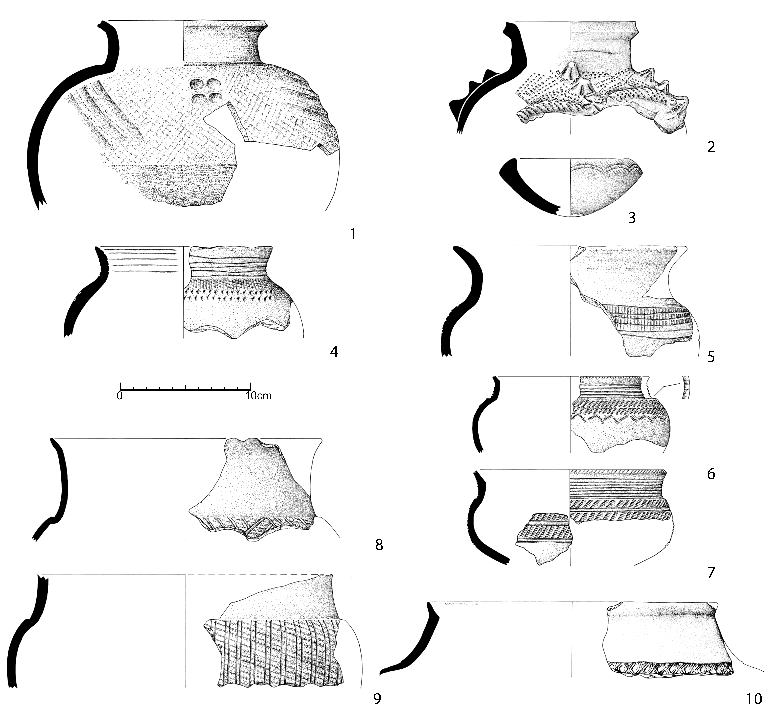
\includegraphics[width=.6\textwidth]{fig/Ngoko-Trad_Typen.pdf}
	\caption{Ceramic vessels of the Ngoko style tradition -- along the rivers Ngoko and Sangha -- that are representative for the following pottery styles: 1--3) Mandombe; 4--5) Konda; 6--7) Ouesso; 8--9) Pandama; 10) Mbenja \citep[145--162]{Seidensticker.2021e}.}
	\label{fig:ngoko}
\end{figure*}

\subsubsection*{Ngoko style tradition}

Between the 13th to 15th centuries CE, a set of ceramics emerged that showed no connection to the Equator-Co tradition and constituted an independent style tradition (Fig.~\ref{fig:ngoko}). Two out of the five pottery groups forming the Ngoko style tradition are dated: the Mandombe style \citep[145--148]{Seidensticker.2021e}, which was defined after the inventory excavated in the upper pit at Pikunda, dates into the 13th to 15th century CE (KI-2891), and the Mbenja style \citep[158--162]{Seidensticker.2021e}, which represents the modern pottery along the upper Sangha and the Ngoko rivers. The other three styles that are part of the Ngoko style tradition can -- thus far -- only be dated relative to these two groups: the Pandama style \citep[155--158]{Seidensticker.2021e} shows considerable similarities with the modern Mbenja pottery, the Quesso style \citep[152--155]{Seidensticker.2021e} shows similarities to the Pandama style, and the Konda group \citep[148--152]{Seidensticker.2021e} shows similarities to the Mandombe and Pandama styles respectively. The proposed order of these pottery styles starts in the 13th to 15th century CE with the Mandombe style, followed by the Kondo group and the Ouesso group, which in turn are surpassed by the Pandama style, which links to the modern Mbenja pottery. All styles share similar main vessel types, pots with convex bellies, concave necks, and short, everted rims. While decorations in the Mandombe style are based on grooves, often using a comb, and comb impressions, the lower halves of the vessels are consistently roughed up by a slurry or slip (Fig.~\ref{fig:ngoko}.1--3). A diagnostic property are plastic decorations, such as knobs and ledges, that can only be found among vessels of the Mandombe group. While relying on grooves and impressions, the succeeding Konda style shows no plastic decoration (Fig.~\ref{fig:ngoko}.4--5). The Ouesso pottery shows decorations made through grooving and comb impressions, similar to the Konda pottery (Fig.~\ref{fig:ngoko}.6--7). At the same time, the shape of the rims is similar to the Pandama style. The decorations of Pandama pottery are based on knotted strip, twisted string, and alternate knotted strip roulettes, which are sometimes superimposed by grooves (Fig.~\ref{fig:ngoko}.8--9). Roulette decoration was previously observed only in some vessel units associated with the Mandombe and Konda styles. This indicates a slow and staged introduction of roulette within the developed system of the Ngoko style tradition \citep[120--123]{Seidensticker.2016b}. Within the modern Mbenja style, vessel shapes become more heterogeneous, with the shape of the rims persisting. Concerning decorations, the Mbenja pottery shows carved roulettes only and decor is restricted to a single band on the vessel’s shoulder (Fig.~\ref{fig:ngoko}.10). Technologically, none of the ceramics associated with the Ngoko style tradition show fabrics, indicative of the usage of fine riverine clays \citep{Seidensticker.2020}. Sherds contain substantial quantities of quartz and organic temper. Sherds of the Mandombe group excavated at Pikunda, and modern pottery produced in Pikunda in 1987, decorated with knotted strip roulette, was produced using coiling. All these styles show inherent commonalities and, at the same time, substantial differences to any pottery linked to the Equator-Co style tradition of the Inner Congo Basin \citep{Wotzka.1995}. The fieldwork of the River Reconnaissance Project in 1987 only uncovered the southern margins of the Ngoko tradition, which reached as far south as Pikunda on the middle Sangha River. Its upstream or northern extent can only be revealed during future fieldwork in the southeast of Cameroon or the southwest of the Central Africa Republic.

\subsection*{Late Iron Age (1000--1850 CE) in the Northern Congo Basin}

The younger part of the pottery sequence in the northern Congo Basin is defined by styles that adopt roulette decoration in an equally staged and slow process as in the Ngoko style tradition. While excavations in this area are rare, only pits with Batalimo-Maluba pottery at Maluba were sufficiently excavated during the River Reconnaissance Project, there are no adequately documented inventories known thus far that yielded pottery dating into the Late Iron Age. Therefore, all lines of reasoning are based on stylistic developments within survey inventories. Modern pottery production documented at four sites on the middle and upper Ubangi river are points of reference for modern ceramics.

At Mbati-Ngombe on the middle Ubangi River, the production of short-necked vessels and bowls with round bases (Fig.~\ref{fig:ubangi}.16--17) shaped via coiling was observed \citep[109-121]{Seidensticker.2021e}. Bowls show inverted rims, while the vessels usually have a short cylindrical neck and very short, everted rim. Most distinctive is the systematic decoration of vessels of the Mbati-Ngombe group using either knotted strip, twisted string, or alternated knotted strip roulettes \citep[88--105]{LivingstoneSmith.2010b} in a single band below the rim or occasionally on the inside of the rim.

Further upstream, ceramic vessels were produced at Dama 1, Sidi and Boduna by pounding in a concave mold \citep[69 Ftn.~101]{Seidensticker.2021e}. Dama style pottery \citep[104--109]{Seidensticker.2021e} consists of either smaller pots with rounded bases and short everted rims but without a defined neck area or substantially bigger vessels with pronounced convex shoulders and everted rims (Fig.~\ref{fig:ubangi}.18--19). The primary means of decoration within the Dama style are carved roulettes, consistently applied in a single band on the vessel’s shoulder. Only rarely is the roulette accompanied by grooves or impressions.

The Kptene style summarizes a set of ethnographic vessels whose production was not documented. This style is comprised of ovaloid vessels and bowls with round bases that are extravagantly decorated with multiple bands of carved roulette \citep[103--105]{Seidensticker.2021e}. Near Bangui, modern vessels with flat bases and a decoration not relying on roulettes are observed \citep[112--114]{Seidensticker.2021e}. This group, named after the capital of the Central African Republic, shows systematic roughing up of the lower parts of the vessels with \textit{bnfwa-nfwa}. In contrast, the upper parts are decorated with multiple bands of impressions and grooves (Fig.~\ref{fig:ubangi}.20).

The most distinctive style among the precursors of these modern productions is the Motenge-Boma group \citep[99--103]{Seidensticker.2021e}, first discovered by Van Noten (\citeyear{vanNoten.1978}, 75, \citeyear{vanNoten.1982a}, 69, Fig.~40). The vessels of the Motenge-Boma group show convex bellies, no pronounced neck areas and, most importantly, a particular variety of rim shapes (Fig.~\ref{fig:ubangi}.12--15). Often, the usually straight or slightly inverted rims show thick ledges. The spectrum of vessel shapes within the Motenge-Boma group also includes convex bows with thickened rims. A clear marker of the Motenge-Boma pottery is a decoration based on bands of carved or, in some cases, knotted strip roulette in combination with grooves and impressions on the bellies and shoulders of vessels. The rims are often also decorated similarly. No new pointers for the dating of the Motengo-Boma pottery have been obtained as studied ceramics of this style were found entirely as surface finds. Thus, until excavations uncover inventories pertaining to this style as well as datable material, the age of the Motenge-Boma pottery can only be estimated to be somewhere in the second half of 2nd millennium CE as suggested by Van Note (\citeyear{vanNoten.1982a}, 69). The detailed surveys of 1985 could demarcate the distribution of this pottery along the Ubangi River quite well. Motenge-Boma ceramics are only found from the mouth of the Lua River in the south to Bangui in the north \citep[102 Fig.~37]{Seidensticker.2021e}.

Evidence for pottery dating between the end of the Batalimo-Maluba style in the 6th century CE (Fig.~\ref{fig:bayes}, \ref{tab:bayes}) and the onset of the Motenge-Boma group is scarce. The styles Dongo, Mokelo and Bobulu \citep[Fig.~\ref{fig:chrono};][86--95]{Seidensticker.2021e} are noteworthy as they date potentially between the mid of the 1st millennium CE and the middle of the 2nd millennium CE. The most diagnostic among these is the Mokelo pottery, distributed between the mouth of the Lua River and the bend of the Ubangi River further upstream. Its vessels often show tapered profiles (Fig.~\ref{fig:ubangi}.8--9). While carved roulette decoration is occasionally present, the bulk of its decors is achieved utilizing incisions and bands of comb impressions.

Notably, no ceramics dating to before the 10th century CE were found along the lower stretches of the Ubangi River, south of Impfondo. All finds from that region pertain to pottery styles known from the Inner Congo Basin, such as Bondongo, Mbandaka, and Botendo \citep[172--181]{Seidensticker.2021e}, with the only exception being the newly described Bokwango style \citep[Fig.~\ref{fig:ubangi}.10--11;][96--99]{Seidensticker.2021e}. The ceramics of this group are an off-shoot for the Equator-Co style tradition \citep{Wotzka.1995}. The lower halves of Bokwango vessels are decorated with \textit{bnfwa-nfwa}, as is typical for styles from the Inner Congo basin dating into the Late Iron Age but showing slightly tapered profiles.

\section*{Discussion}

\subsection*{Settlement History of the Congo Basin}

The results from the northern and western parts of the Congo Basin presented here complement the available data on the settlement history of the Inner \citep{Wotzka.1995} and Eastern Congo Basin \citep{LivingstoneSmith.2017}, enabling a synopsis of the settlement history of the region as a whole \citep[218--244]{Seidensticker.2021e}. The earliest pottery group known within the entire Congo Basin thus far is the Imbonga style, dating into the 4th to 2nd century BCE (Fig.~\ref{fig:bayes}; \ref{fig:chrono}; Tab.~\ref{tab:bayes}) and is found within the western half of the Inner Congo Basin \citep[Fig.~\ref{fig:timeslices};][59--68]{Wotzka.1995} as well as at two sites along the lower Sangha river.

The Imbonga style differentiates into multiple groups that still inherit substantial morphological and decoration characteristics in the following phase, starting in the 3rd and 2nd century BCE \citep[219--224]{Seidensticker.2021e}. Initially, the later individually described styles Bonkake, Ingende and Inganda \citep[Fig.~\ref{fig:bayes}; \ref{fig:chrono}; Tab.~\ref{tab:bayes};][68--84]{Wotzka.1995} were conceptualized as part of a broader ‘Imbonga horizon’ \citep{Eggert.1983}. During this time, the settled area in the Inner Congo Basin slightly expanded upriver along the lower Tshuapa, up to the region of the modern town of Boende, and on the lower Luilaka (Fig.~\ref{fig:timeslices}). The development of ceramic styles in the Inner Congo Basin around the turn of time is characterized by differentiation and regionalization, with many of the successors of the Imbonga style being only distributed along certain tributaries of the Congo River.

Around the same time, the initial settlement phase of pottery-producing communities starts in the western and northern Congo Basin. Along the Sangha and Likwala-aux-Herbes rivers, the Pikunda-Munda style emerges. Along the middle Ubangi River, on the northern fringes of the rainforest, the Batalimo-Maluba (Fig.~\ref{fig:bayes}; \ref{fig:chrono}; Tab.~\ref{tab:bayes}) and the Ngbanja styles can be found (Fig.~\ref{fig:timeslices}). It is essential to state that these groups share no fundamental commonalities with the pottery of the Inner Congo Basin and must be regarded as distinct and individual lines of development. Based on preliminary technological analyses, a connection to the Inner Congo Basin's contemporaneous ceramics can only be postulated for the Pikunda-Munda group. Ceramics within the western and Inner Congo Basin appear to have been shaped in either a drawing of a lump or a ring technique. These ceramics have yet to be differentiated, especially regarding used clays and the lack of tempering of the clays \citep{Seidensticker.2020}. 

Also within time period, the initial phase of pottery-producing communities emerged in the north-eastern parts of the Basin, in the vicinity of Kisangani \citep[Fig.~\ref{fig:timeslices};][]{LivingstoneSmith.2017}. The pottery of the Early Phase dates between the 2nd century BCE and 1st century CE (Fig.~\ref{fig:bayes}; \ref{fig:chrono}; Tab.~\ref{tab:bayes}). It shares some similarities with the contemporaneous styles of the Inner Congo Basin, such as using similar decorative elements like rocker zigzag with a comb on the bottom parts of vessels and flat bases. An equally close or even closer comparison between the pottery of the Early Phase in the Eastern Congo Basin can be made to the Ngbanja style found along the Ubangi river \citep[204--205]{Seidensticker.2021e}. The ovoid shapes with flat bases, everted rims, and decorations on the vessels’ shoulders are reminiscent of the Ngbanja style. The early ceramics from the Kisangani region also lack systematic decoration of the lower parts with rocker zig-zag with a comb and plastic elements such as knobs or ledges, both predominant markers of the Imbonga style \citep[59--68]{Wotzka.1995}. Pottery of the Early Phase is still attested until the 1st century CE, while the Middle Phase pottery already commences \citep[Fig.~\ref{fig:bayes}; \ref{fig:chrono}; Tab.~\ref{tab:bayes};][]{LivingstoneSmith.2017}.

The first half of the 1st millennium CE sees a continuation of the described patterns. In the Inner Congo Basin, multiple interrelated styles with only regional distribution areas emerge (Fig.~\ref{fig:timeslices}). It should be remarked that during this time, a slight retreat of settlement activity is discernible, with substantially fewer sites compared to the centuries BCE being known along the Lulonga and Lopori rivers \citep[224]{Seidensticker.2021e}. This plateauing of settlement activity led to the setback in human activity visible throughout Central Africa that continued until the 10th century CE \citep{Seidensticker.2021}.

\begin{figure*}[!tbp]
	\centering
	\includegraphics[width=\textwidth]{fig/fig_chronology.pdf}
	\caption{Temporal distribution of known pottery styles in the Congo Basin over the past 2600 years separated by regions \citep[Fig. 1; D) Norther Congo Basin, E) Western Congo Basin, F) Inner Congo Basin, G) Eastern Congo Basin]{Seidensticker.2021}. Circles represent the highest probability of calibrated calendar age of each pottery-linked 14C date. The intensity of grey-shading is proportional to the summed probability of the calendar-age windows of all pottery occurrences by type. Colored bars represent the phase duration of radiocarbon dates pottery styles. For groups with more than two associated radiocarbon dates, the median start and end dates of the phases were calculated using a Bayesian phase model (Fig.~\ref{fig:bayes}, Tab.~\ref{tab:bayes}). Dashed colored bars indicate estimated 100-year bins derived from stylistic resemblance \citep[Data S2]{Seidensticker.2021}.}
	\label{fig:chrono}
\end{figure*}

\begin{figure*}[!tbp]
	\centering
	\includegraphics[width=\textwidth]{fig/fig_map_time_slices.pdf}
	\caption{Time-sliced maps of occurrences of pottery styles in the Congo Basin. Negative numbers indicate calibrated ages BCE, while positive numbers represent calibrated ages CE. Extend per type was calculated as concave hull \citep{Gombin.2017} with a buffer of 20~km. The extent of the map is equal to Figure \ref{fig:map} and colors correspond to Figure \ref{fig:chrono}.}
	\label{fig:timeslices}
\end{figure*}

Within the entire Congo Basin, only very few sites point to the presence of pottery-producing communities between the 7th to 10th centuries CE (\citeauthor{Seidensticker.2021e} \citeyear{Seidensticker.2021e}, 225--231; \citeauthor{Seidensticker.2021} \citeyear{Seidensticker.2021}, Fig. S4). The two predominant styles in the western and northern Congo Basin, the Pikunda-Munda and Batalimo-Maluba groups, end between the 4th to 6th century CE at the latest (Fig.~\ref{fig:bayes}, Tab.~\ref{tab:bayes}). The available dates for the Middle Phase pottery in the Kisangani region indicate that it ended around the same time. The earliest evidence for the Ilambi style, clearly pertaining to the younger Iron Age, dates to the 8th century CE \citep[98 Tab.~1]{LivingstoneSmith.2017}. It must be stressed that this early date is challenged by another date also associated with the Ilambi style, dating into the 15th to 17th century CE, leaving a considerable discrepancy.

Substantial human activity is attested for again by significant increases in sites yielding pottery dating to the 11th century CE and younger. Among these are the widely distributed Bondongo and Longa styles \citep[Fig.~\ref{fig:bayes}; \ref{fig:chrono}; Tab.~\ref{tab:bayes};][121--139]{Wotzka.1995}. While these groups are distributed across nearly all parts of the Inner Congo Basin that was surveyed during the River Reconnaissance Project, and in the case of the Bondongo group also along the lower Ubangi river, they are immediately followed by a distinct development of regional traditions (\citeauthor{Wotzka.1995} \citeyear{Wotzka.1995} 221--223; \citeauthor{Seidensticker.2021e} \citeyear{Seidensticker.2021e}, 231–-244; \citeauthor{Seidensticker.2021} \citeyear{Seidensticker.2021}, 3--5). Along the lower Sangha River, the newly dated Ngombe group (Tab.~\ref{tab:14C}) reflects an uptick in human activity. Starting in the 13th century CE, new components of pottery production commence along the Ngoko river and upstream parts at the Sangha river. These new elements form the foundation for the newly described Ngoko style tradition, whose onset is marked by the emergence of the Mandombe style. This group is later followed by at least three more pottery styles that lead directly into the modern potters’ production in the area. Along the Likwala-aux-Herbes River, re-settlement is only attested for starting in the 16th century CE, documented by newly obtained radiocarbon dates for ceramics of the Ebambe style (Tab.~\ref{tab:14C}; RICH-30866). Within a similar time falls the Motenge-Boma style found along the middle Ubangi River. It is putatively preceded by the poorly attested Dongo, Mokelo, and Bobulu groups. The introduction of roulette decoration within the Ngoko style tradition, as well as among the groups on the middle Ubangi river, while being an easily observable maker, cannot be described as a watershed event but rather a process of slow adaption \citep[120--123]{Seidensticker.2016b}. Similarly to these regions, roulette decoration becomes a prime marker of younger pottery styles in the Kisangani region \citep{LivingstoneSmith.2017}. 

\subsection*{Refuting the Sangha River Interval (SRI) Hypothesis}

The putative origin of the ceramic-producing communities starting to settle in the Congo Basin in the 4th century BCE remain elusive. Linguistic studies \citep{Grollemund.2015,Bostoen.2015,Koile.2022,Grollemund.2023} propose rapid migrations through the rainforest and suggest that the region of the Sangha river played a crucial role as a potential gateway into the equatorial rainforest of Central Africa and the Congo Basin. The Sangha River Interval (SRI), ecologically identified as "forest perturbations" seen as a "link between the Sudanian and Zambezian savannas" \citep[356]{Bostoen.2015} was first brought forward in René \cite{Letouzey.1968}. This roughly 400~km wide region between 14 and 18°E "lacks some plant species typical of dense humid forests present in both the lower Guinean and the Congolian floristic domains in Cameroon-Gabon and the Democratic Republic of the Congo, respectively" \citep[356]{Bostoen.2015}. While \cite{Grollemund.2015} and \cite{Bostoen.2015} gain their hypotheses mainly based on statistical analyses of present-day languages, they attempt to integrate archaeological data into their synthesis. It must be noted that both integrations are instead based on cherry-picking than a critical evaluation of the existing archaeological knowledge. The most striking testament of this is the compilation of discussed sites by \citeauthor{Bostoen.2015} (\citeyear{Bostoen.2015}, 356 Fig.~1), depicting only the site of Imbonga on the Momboyo river in the entire Congo Basin. While both papers offer synthesis with far-reaching implications, the available reports of the settlement history of the Sangha region \citep{Eggert.1992,Eggert.1993} were largely omitted. Bostoen et al. (\citeyear{Bostoen.2015}, 364) reduce these reports to a short mention concerning the association of evidence for iron metallurgy with the Pikunda-Munda style. None of the available data, including all radiocarbon dates published by \cite{Eggert.1992,Eggert.1993} and showing at least 200 years off-set between the oldest dates in the heart of the rainforest (Imbonga) versus the oldest dates from within the SRI (Pikunda-Munda; Fig.~\ref{fig:bayes}; Tab.~\ref{tab:bayes}), were integrated into the overall analysis. The entire settlement history of the Inner Congo, which was published in all detail \citep{Eggert.1984,Eggert.1987c,Wotzka.1995}, has been reduced to the putative and untested connection between the earliest pottery style (Imbonga) and the earliest immigration of Bantu speakers \citep[366]{Bostoen.2015}. The more recent studies of \cite{Koile.2022} and \cite{Grollemund.2023} upheld the same basic argumentation and failed to integrate historical evidence procured through archaeology properly.

Recent paleo-ecological field data from within the SRI \citep{Bremond.2017} refute also the paleo-environmental assumptions made by \cite{Grollemund.2015} and \cite{Bostoen.2015}. While the biogeographical concept goes back to \cite{Letouzey.1968} and the unique composition of the forest in the Sangha region being discernible even in modern remote sensing data \citep{Gond.2013,Philippon.2019}, ground truths for a widespread opening of the forest in that region are lacking. A recent analysis questioned the existence of the SRI as an ecological phenomenon \citep{Bremond.2017}. The study relied on a multi-proxy analysis, combining phytolith assemblages with d13C rations of the soil organic carbon from 18 soil profiles within the SRI. Out of all 18 profiles, only four showed d13C values higher than -25 ‰ and can be related to past vegetation changes during the 1st millennium BCE. The phytolith assemblages \citep[99]{Bremond.2017} further corroborate these findings of only occasional and rare forest openings. Paleo-environmental data do not sustain the notion of an opening up of the SRI. Paleo-environmental data do not sustain the notion of an opening up of the SRI. In conclusion, the SRI has to be considered a patchy opening of the dens forest rather than a 'Savannah corridor', and the fact that pottery-producing communities settled within it at least 200 years after the Inner Congo Basin was already settled dismisses the argumentation brought forward by \cite{Grollemund.2015} and \cite{Bostoen.2015}.

\subsection*{Middle Iron Age Hiatus in the Congo Basin}

Of equal importance to the onset of the settlement of the Congo Basin by pottery-producing communities is the persistence of these communities over the past 2400 years. As mentioned, an extensive reduction or nearly complete discontinuation of settlement activities was reported earlier for Gabon by Oslisly (\citeyear{Oslisly.1998}, 101--103 Fig.~9, \citeyear{Oslisly.2001d}, 112--113 Fig.~7.9). \cite{Leka.2008} reported an interruption of settlement activities at sites north of Yaoundé (Cameroon) between the 1st and 10th century CE. Dibamba, with six hectares the biggest site in the region in terms of examined surface, showed a hiatus between the 4th and 10th centuries CE \citep{Saulieu.2017}. An interruption of the local pottery sequence was also observed on the well-studied island of Corisco (Equatorial Guinea) \citep[355--356]{SanchezElipe.2016}. Here, after the end of the late Oveng pottery in the 8th century CE, ceramics and other archaeological features have been missing for about 200 years until the onset of the Nandá pottery in the 10th/11th century CE. The bigger trend has been discussed recently \citep{deSaulieu.2021a,Seidensticker.2021}.

The sequence of pottery styles in the Inner Congo Basin has been described as uninterrupted by \cite{Wotzka.1995}. A detailed review of chronological indicators for the 32 pottery styles described by Wotzka (\citeyear{Wotzka.1995}, 59--212) revealed that no pottery could be securely dated between the end of the Bokuma and Lingonda styles, which come to an end in the 7th centuries CE at the latest, and the onset of the widespread Bondongo style at the beginning of 12th century CE (Fig.~\ref{fig:bayes}; Tab.~\ref{tab:bayes}). The Longa style was proposed to be potentially dated in-between the Early and Late Iron Age \citep[121–-128]{Wotzka.1995}. None of the three radiocarbon dates associated with Longa pottery date into the time-span between the 6th to 10th century CE. Two somewhat older dates (Hv-12611, Hv-12626) are discarded by Wotzka (\citeyear{Wotzka.1995}, 127--128 Tab. 53) as not-representative. The third available date (Hv-11572) covers the 11th to 14th century CE. This last date goes very well with the close stylistic connections Longa pottery shows to the Bondongo style, which is firmly dated between the beginning of the 12th and the end of the 14th century CE \citep[Fig.~\ref{fig:bayes}; \ref{fig:chrono}; Tab.~\ref{tab:bayes};][138 Tab.~58]{Wotzka.1995}. The younger date for the Longa pottery is further supported by a new radiocarbon dating obtained from a food crust on the bottom of the enormous globular vessel found at Ngombe on the middle Sangha river (Tab.~\ref{tab:14C}; RICH-30867). The ceramics found within this feature are the basis of the pottery style of the same name, which shows extreme similarities with the Longa style. This gives enough reason to propose the age of the Longa style to be later than the 10th century CE, thus dating it firmly to the Late Iron Age. Consequently, this reassessment of the chronology of the Longa pottery leaves the same ‘gap’ or ‘hiatus’ within the sequence of the Inner Congo Basin that has been observed all over the Congo Basin \citep{deSaulieu.2021a,Seidensticker.2021}. Consequently, the conceptualization of an uninterrupted sequence of pottery styles starting with the Imbonga style and leading, similar to a network of direct decedents, right to the local potters’ producing ceramic today \citep[65, 221, 274, 285]{Wotzka.1995} must be questioned.

\subsection*{Fuzzy Border at the Ubangi river}

Another intriguing aspect concerns the importance of the surveyed river systems. Particular focus is always laid on whether rivers constitute exchange barriers or, instead, if they are preferred pathways for expansion and axes of contact \citep{Russell.2014}. The observed distribution patterns of pottery styles along the Ubangi river, a consecutive 850~km long north--south transect, show a seemingly impermeable border zone that existed for nearly two millennia \citep[183--185, 184 Tab.~17]{Seidensticker.2021e}. These zones are persistent and long-lasting, with ceramics rarely found outside their specific region. This 'fuzzy' boundary is situated between 1° to 1.5°~N, north of Impfondo. South of this region, all ceramics date into the Late Iron Age and are all associated with the Equator-Co style tradition of the Inner Congo Basin \citep{Wotzka.1995}. Further upriver, near the mouth of the Lua river, the Batalimo-Maluba style is among the earlier potteries in the region. All pottery groups that follow afterwords 'respect' the southern border of the Batalimo-Maluba group (Fig.~\ref{fig:timeslices}). This observation offers a unique view into a putative lack of social connectivity along one of the major rivers in Central Africa and needs more research.

\section*{Conclusions}

While pottery styles identified in the northern parts of the study area follow independent trajectories, the styles of the western parts of the Congo Basin show substantial similarities to contemporaneous styles from the Inner Congo Basin. These similarities start with the clay sourcing, resulting in very similar macroscopic ceramic fabrics. Furthermore, while vessel shapes are sometimes different, decorations techniques and motives are nearly identical. Concerning the Pikunda-Munda style, the oldest pottery widely distributed in the western Congo Basin, strong technological similarities stand in the way of several stylistic differences. So far, this style can only be loosely associated with contemporaneous ceramics of the Inner Congo Basin. Furthermore, the Pikunda-Munda style did not develop into an individual stylistic tradition, and after its end, there are no reliable links with any younger styles in the region. More critical for the settlement history of the Congo Basin is the fact that the emergence of the Pikunda-Munda group can only be dated as about 300 years younger than the emergence of the first pottery production further east, in the Inner Congo Basin. This fact, also considering that it is the earliest widely distributed pottery in the Sangha River Interval and shows legitimate stylistic differences to the ceramics from the Inner Congo Basin, the prevailing hypothesis of the Sangha River Interval must be rejected from an archaeological perspective.

After the setback in human activity during the 7th to 10th centuries CE, pottery groups such as the Ngombe style appear that show close stylistic ties to pottery from the Equator Co-Tradition and can be regarded as part of them. The same general association as western offshoots of the Equator Co-Tradition goes for the younger styles Ebambe and Epena.

The introduction of roulette decorations, which often govern decoration practices of modern-day ceramics, is equally vital for the region's settlement history. A gradual adoption and intensive use of this ornamentation practice can be observed within the Ngoko tradition. In the extreme south of the study area, another distinct line of pottery development was observed within the grog-tempered Bobusa group.

The settlement sequence of the northern and western Congo Basin sketched out within this study must, at least in part, be taken cautiously due to the limited sources available. Only new fieldwork and excavations can remedy this situation. Thus far, the available data constitutes valid proof for the chrono-temporal position of the early parts of the sequence during the Early Iron Age. However, available data from the middle of the 1st millennium CE onwards must be considered incomplete. Despite the extensive body of material obtained by the River Reconnaissance Project in the 1980s, the present work only provides a first insight into the ceramic variability of the region.

\begin{acknowledgements}
Thanks go to Manfred K. H. Eggert for granting access to the finds from this project and supporting the research. Additional thanks go to Hans-Peter Wotzka for advising the research from 2012 to 2016 and Thomas Knopf for his supervision afterwards. Katharina Jungnickel deserves thanks for commenting on an earlier draft of this paper.

Newly obtained radiocarbon dates on food crusts, dated at the radiocarbon dating laboratory of the Royal Institute for Cultural Heritage in Brussels (RICH) and funded by the FWO postdoctoral scholarship (1287922N) granted to the author.

All data and computer code generated during this research is available here: \url{https://github.com/dirkseidensticker/PikundaMunda_BatalimoMaluba_AAR}.
\end{acknowledgements}

\bibliographystyle{spbasic}
\bibliography{references.bib}

\end{document}
